\documentclass[aspectratio=43]{beamer}

\usetheme{PaloAlto}
\usecolortheme{default}
\usefonttheme[onlymath]{serif}

\usepackage[alf]{abntex2cite}
\usepackage[brazil]{babel}
\usepackage{color}
\usepackage[T1]{fontenc}
\usepackage{graphicx}
\usepackage[utf8]{inputenc}
\usepackage{txfonts}
\usepackage{comment}


\title{Proposta de melhoria de desempenho do SIGA utilizando Nginx como 
servidor HTTP}
\author{Lucas Rafael Araujo Andrade}
\institute{
Orientador: Alexandre Ramos Fonseca \\
Universidade Federal dos Vales do Jequitinhonha e Mucuri - UFVJM
\par
Faculdade de Ciências Exatas e Tecnológicas - FACET
\par
Departamento de Computação - DECOM
\par
Bacharelado em Sistemas de Informação}
\date{15 de Dezembro de 2014}


% ----------------- INÍCIO DO DOCUMENTO --------------------------------------
\begin{document}

% ----------------- CAPA --------------------------------
\begin{frame}

\titlepage

\end{frame}
% ----------------- SUMÁRIO --------------------------------
\begin{frame}{Sumário}
\tableofcontents
\end{frame}

% ----------------- INTRODUÇÃO --------------------------------

\begin{frame}
	\centering
	{\Huge Introdução}
\end{frame}

\section{Introdução}\label{sec:introducao}

% ----------------- SLIDE 1 --------------------------------

\begin{frame}{Introdução}
	\begin{block}{}
		\begin{itemize}
			\item Avanço dos computadores e redes de comunicação;
			\item Computadores pessoais ---> Servidores \textit{web};
			\item Acessíveis no mundo todo;
			\item Servidores HTTP.
		\end{itemize}
	\end{block} \pause
	\begin{block}{}
		\begin{itemize}
			\item Conteúdo dinâmico;
			\item Ambientes chegando ao limite;
			\item Fragilidades expostas;
			\item Falta desempenho.
		\end{itemize}
	\end{block}
\end{frame}
% ----------------- SLIDE 2 --------------------------------
\begin{frame}{Escalabilidade}
	\begin{block}{Escalabilidade}
		``Escalabilidade é um atributo desejável de 
		uma rede, sistema ou processo.'' (BONDI, 2000).
		\begin{itemize}
			\item Acomodar uma quantidade sempre maior de elementos ou objetos; 
			\pause
			\item Processar quantidade crescente de trabalho; \pause
			\item Suscetível a ampliação;
		\end{itemize}
	\end{block}
\end{frame}
% ----------------- SLIDE 3 --------------------------------
\begin{frame}{Escalabilidade}
	\begin{block}{Escalabilidade}
		Quando se diz que um sistema não é escalável ou que não escala:
		\begin{itemize}
			\item Custo adicional é excessivo; \pause
			\item Tempo de resposta; \pause
			\item Processamento (processador); \pause
			\item Espaço; \pause
			\item Memória; \pause
			\item Dinheiro.
		\end{itemize}
	\end{block}
\end{frame}
% ----------------- SLIDE 4 --------------------------------
\begin{frame}{Escalabilidade}
	\begin{block}{Escalabilidade}
		\begin{itemize}
			\item É crucial para o sucesso à longo prazo de um sistema; \pause
			\item Pode ser comprometida por ações repetidas de forma frequente; 
			\pause
			\item Algoritmos que levem a \textit{deadlock}; \pause
			\item Escalonamento de recursos ruim.
		\end{itemize}
	\end{block}
\end{frame}
% ----------------- SLIDE 5 --------------------------------
\begin{frame}{SIGA}
	\begin{block}{SIGA}
		\begin{itemize}
			\item Adquirido em 2007 da UFJF; \pause
			\item PHP e Miolo; \pause
			\item Apache HTTP \textit{Server}.
		\end{itemize}
	\end{block} \pause
	\begin{block}{Apache}
		\begin{itemize}
			\item Desenvolvido desde 1.995;
			\item Mais utilizado desde então;
			\item Aproximadamente 37\% dos sítios no mundo.
		\end{itemize}
	\end{block}
\end{frame}
% ----------------- SLIDE 6 --------------------------------
\begin{frame}{Utilização dos Servidores \textit{Web}}
	\begin{figure}
		\centering
		\caption{Utilização de Servidores \textit{web} no mundo}
		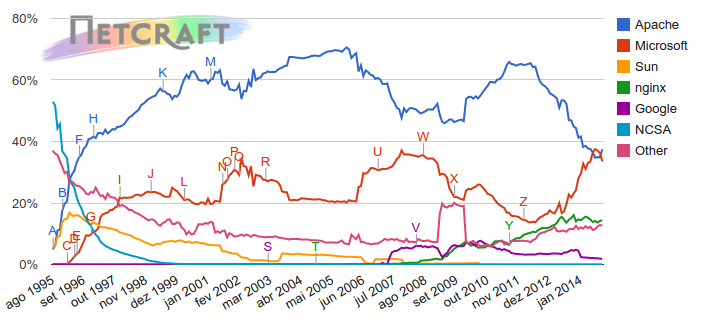
\includegraphics[width=1\linewidth]{../figuras/grafico1}\\
		Fonte: Netcraft
	\end{figure}
\end{frame}
% ----------------- SLIDE 7 --------------------------------
\begin{frame}{Utilização dos Servidores \textit{Web}}
	\begin{figure}
		\centering
		\caption{Utilização de Servidores \textit{web} entre os 1.000.000 de 
		sítios 
		}
		mais acessados no mundo.
		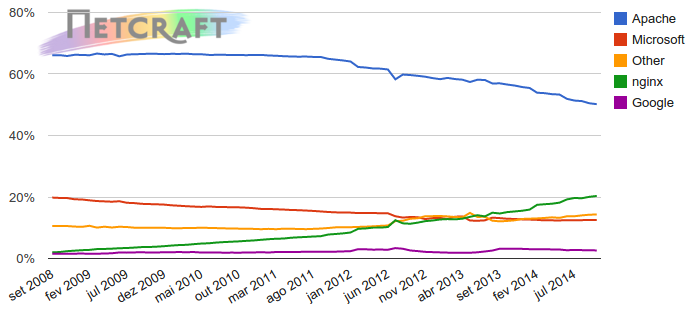
\includegraphics[width=1\linewidth]{../figuras/grafico2} \\
		Fonte: Netcraft
	\end{figure}
\end{frame}
% ----------------- SLIDE 8 --------------------------------
\begin{frame}{Utilização dos Servidores \textit{Web}}
	\begin{itemize}
		\item Queda na utilização do Apache; \pause
		\item Aumento da utilização do Nginx; \pause
		\item Tecnologia em ascensão não significar ser melhor; \pause
		\item Investigar é necessário.
	\end{itemize}
\end{frame}

\subsection*{Motivação}
% ----------------- SLIDE 9 --------------------------------
\begin{frame}{Motivação}
	\begin{itemize}
		\item Aumento do número de usuários; \pause
		\item Lentidão eventual do sistema; \pause
		\item 3.500 novos alunos por ano.
	\end{itemize}
\end{frame}
% ----------------- SLIDE 10 --------------------------------
\begin{frame}{Motivação}
	\framesubtitle{Pessoas ligadas à UFVJM}
	\centering
	\begin{table}
		\caption{Pessoas ligadas à UFVJM}
		\begin{tabular}{|c|c|}
			\hline
			Alunos & 8.121 \\ \hline
			Professores & 576 \\ \hline
			Servidores Técnico-Administrativo & 421 \\ \hline
			\textbf{Total} & 9.118 \\ \hline
		\end{tabular}
	\end{table}
	Fonte: UFVJM Em Números
\end{frame}
% ----------------- SLIDE 11 --------------------------------
\begin{frame}{Motivação}
	\framesubtitle{Dez dias com mais acessos ao SIGA}
	\centering
	{\small \begin{table}
		\caption{Dez dias com mais acessos no SIGA}
		\begin{tabular}{|c|c|c|}
			\hline
			\textbf{Dia} & \textbf{Acessos}  & \textbf{Ocasião} \\ \hline
			16/08/2014 & 20.942 & Início da Pré Matrícula \\ \hline
			25/08/2014 & 17.536 & Início do Período Letivo \\ \hline
			16/04/2013 & 17.091 & Dias Finais do Período Letivo \\ \hline
			30/09/2013 & 17.007 & Início da Pré Matrícula \\ \hline
			17/04/2013 & 16.772 & Dias Finais do Período Letivo \\ \hline
			15/04/2013 & 16.597 & Dias Finais do Período Letivo \\ \hline
			31/07/2014 & 16.035 & Dias Finais do Período Letivo \\ \hline
			29/07/2014 & 15.744 & Dias Finais do Período Letivo \\ \hline
			28/07/2014 & 15.477 & Dias Finais do Período Letivo \\ \hline
			30/07/2014 & 14.854 & Dias Finais do Período Letivo \\ \hline
		\end{tabular}
	\end{table}}
	Fonte: Base de Dados do SIGA
\end{frame}

\subsection*{Objetivos}
% ----------------- SLIDE 12 --------------------------------
\begin{frame}{Objetivos}
	\begin{block}{Objetivo Geral}
		Identificar se a utilização do servidor HTTP Nginx é mais eficiente do 
		que o utilizado atualmente, o Apache HTTP \textit{Server}.
	\end{block} \pause
	\begin{block}{Objetivos Específicos}
		Analisar os dados coletados a partir de testes realizados para 
		identificar se o Nginx é mais eficiente do que o Apache; apresentar a 
		solução encontrada e analisar o que pode ser feito para evitar a 
		substituição ou reconstrução do SIGA.
	\end{block}
\end{frame}

% ----------------- FUNDAMENTAÇÃO TEÓRICA --------------------------------

\section*{}
\begin{frame}
	\centering
	{\Huge Fundamentação Teórica}
\end{frame}

\section{Fundamentação Teórica}\label{sec:fundamentacao-teorica}

\subsection*{Aplicação Cliente/Servidor}

% ----------------- SLIDE 14 --------------------------------
\begin{frame}{Cliente/Servidor}
	\begin{block}{Cliente}
		``Um solicitante de informações em rede, normalmente um computador ou 
		estação de trabalho, que pode consultar o banco de dados e/ou outras 
		informações de um servidor.'' (STALLINGS, 2005)
	\end{block}
	\begin{block}{Servidor}
		``Um computador, normalmente uma estação de trabalho poderosa ou um 
		\textit{mainframe} que abriga informações para manipulação por clientes 
		em rede.'' (STALLINGS, 2005)
	\end{block}
\end{frame}
% ----------------- SLIDE 15 --------------------------------
\begin{frame}{Aplicações Cliente/Servidor}
	\begin{itemize}
		\item Conjuntos de programas no cliente e servidor; \pause
		\item Solicitações partem do cliente; \pause
		\item Servidor provê o recurso; \pause
		\item Geralmente utilizam o protocolo HTTP; \pause
		\item Muito utilizados na construção de sistemas informação.
	\end{itemize}
\end{frame}

% ----------------- SLIDE 16 --------------------------------

\begin{comment}
\begin{frame}{Protocolo}
		\begin{block}{Definição de Protocolo}
		\begin{enumerate}
			\item Ata, nota ou registro dos documentos governamentais, dos 
			atos oficiais, da correspondência de um governo ou tribunal, de uma 
			empresa, universidade etc.
			\item Subdivisão de uma repartição pública (ou empresa privada) em 
			que se registram e/ou se recebem os requerimentos, documentos ou 
			processos.
			\item Recibo que registra o número e a data em que um processo ou 
			requerimento foi catalogado e registrado.
			\item Acordo regulamentado entre países ou empresas: protocolo 
			internacional.
		\end{enumerate}
	\end{block}
\end{frame}
\end{comment}

\subsection*{Protocolo de Comunicação}

\begin{frame}{Protocolo de Comunicação}
	\begin{itemize}
		\item Convenção; \pause
		\item Controla e possibilita conexão, comunicação e transferência; 
		\pause
		\item Sintaxe: Inclui elementos como formato de dados e níveis de 
		sinal; \pause
		\item Semântica: Inclui informações de controle para coordenação e 
		tratamento de erro; \pause
		\item Temporização: Inclui combinação de velocidade e sequência.
	\end{itemize}
\end{frame}

% ----------------- SLIDE 18 --------------------------------
\subsection*{TCP/IP}

\begin{frame}{TCP/IP}
	\begin{block}{TCP/IP}
		\begin{itemize}
			\item Conjunto de protocolos; \pause
			\item Organizados em camadas; \pause
			\item Cinco camadas.
		\end{itemize}
	\end{block}
\end{frame}
% ----------------- SLIDE 19 --------------------------------
\begin{frame}
	\begin{block}{Camadas TCP/IP}
			\centering
			\begin{table}
				\begin{tabular}{|c|}
					\hline
					\textbf{Camadas} \\ \hline
					Aplicação \\ \hline
					Transporte \\ \hline
					Rede \\ \hline
					Enlace\\ \hline
					Física\\ \hline
				\end{tabular}
			\end{table}
	\end{block}
\end{frame}


% ----------------- SLIDE 20 --------------------------------
\subsection*{Protocolo HTTP}

\begin{frame}{Protocolo HTTP}
	\begin{itemize}
		\item Protocolo básico da WWW; \pause
		\item Camada de aplicação; \pause
		\item Pode ser usada em qualquer aplicação cliente/servidor. \pause
		\item Transferir texto, hipertexto, áudio, imagem, etc.
	\end{itemize}
\end{frame}

% ----------------- TECNOLOGIAS UTILIZADAS --------------------------------

\section*{}
\begin{frame}
	\centering
	{\Huge Tecnologias Utilizadas}
\end{frame}

\section{Tecnologias Utilizadas}\label{sec:tecnologias-utilizadas}

\subsection*{Apache HTTP Server }

\begin{frame}{Apache}
	\begin{block}{Apache}
	\begin{itemize}
		\item Servidor HTTP;
		\item Lançado em 1.995;
		\item Servidor mais utilizado atualmente.
	\end{itemize}
\end{block}
\end{frame}

\subsection*{Nginx}

\begin{frame}{Nginx}
	\begin{block}{Nginx}
	\begin{itemize}
		\item Servidor HTTP;
		\item Criado em 2.002 e publicado em 2.004;
		\item Arquitetura orientada à eventos e assíncrona;
		\item Utiliza quantidades pequenas e previsíveis de memória;
		\item Utilizado por vários sítios de alto tráfego.
	\end{itemize}
\end{block}
\end{frame}

\subsection*{ApacheBench}

\begin{frame}{ApacheBench}
	\begin{block}{ApacheBench}
	\begin{itemize}
		\item Criado em 1.996;
		\item Ferramenta para comparar desempenho dos servidores Apache;
		\item Funciona para qualquer servidor HTTP.
	\end{itemize}
\end{block}
\end{frame}

\subsection*{FastCGI}

\begin{frame}{FastCGI}
	\begin{block}{FastCGI}
	\begin{itemize}
		\item Interface de comunicação para servidores \textit{web};
		\item Combina o melhor do CGI e API's proprietárias;
		\item Executa processos de forma separada e isolada;
		\item Desempenho, simplicidade, Independência de linguagem e 
		arquitetura, isolamento de processos, suporte a computação distribuída.
	\end{itemize}
\end{block}
\end{frame}

\subsection*{HTML}

\begin{frame}{HTML}
	\begin{block}{HTML}
	\begin{itemize}
		\item Linguagem de marcação;
		\item Baseado no conceito de hipertexto;
		\item Publicação de conteúdo;
		\item Independente de plataforma.
	\end{itemize}
\end{block}
\end{frame}

\subsection*{PHP}

\begin{frame}{PHP}
	\begin{block}{PHP}
	\begin{itemize}
		\item Linguagem de programação;
		\item Interpretada, de propósito geral, tipagem dinâmica e 
	fraca, procedural, reflexiva, orientada a objetos e funcional;
		\item Melhor usada na criação de sistemas \textit{web};
	\end{itemize}
	\end{block}
\end{frame}

% ----------------- METODOLOGIA --------------------------------

%\section{Metodologia}\label{sec:metodologia}

\begin{frame}{Coleta dos Dados}
	\begin{itemize}
		\item Ferramenta ApacheBench;
		\item ``ab -n X -c Y'';
		\item X = Requisições Totais;
		\item Y = Requisições Simultâneas.
	\end{itemize}
\end{frame}

\begin{frame}{Ambiente de Testes}
	\begin{block}{Máquinas Virtuais}
		\begin{itemize}
			\item VirtualBox;
			\item Debian 7;
			\item 2GB de RAM;
			\item 30GB de HD;
			\item 1 Núcleo.
		\end{itemize}
	\end{block} \pause
	\begin{block}{Hospedeiro}
		\begin{itemize}
			\item Computador Portátil;
			\item Intel Core i5-3337U @ 1,8Ghz - 4 Núcleos;
			\item 8GB de RAM;
			\item 1TB de HD.
		\end{itemize}
	\end{block}
\end{frame}

\begin{frame}{Definição Dos Valores Utilizados nos Testes}
	\begin{block}{Valores}
		\begin{itemize}
			\item Requisições Totais variando de 1.000 à 15.000 com salto de 
			1.000;
			\item Carga de 10, 20, 40 e 80 porcento.
		\end{itemize}
	\end{block}
\end{frame}

\begin{frame}{Definição Dos Valores Utilizados nos Testes}
	\begin{figure}
		\centering
		\caption{Requisições Totais e Requisições Concorrentes}
		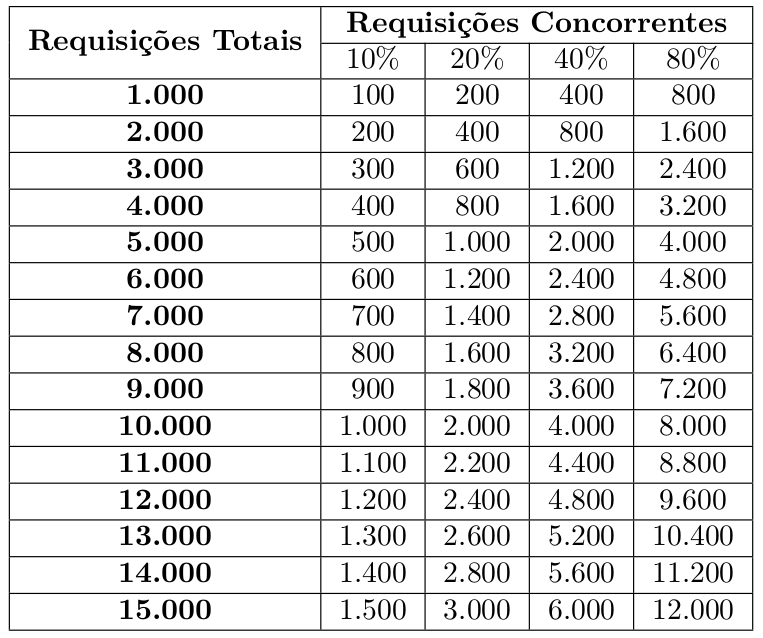
\includegraphics[width=0.7\linewidth]{tabela-requisicoes} \\
	\end{figure}
\end{frame}

\begin{frame}{Métricas Utilizadas}
As métricas utilizadas para comparar o desempenho dos servidores HTTP são as 
mesmas métricas calculadas e entregues pelo ApacheBench.
\begin{block}{Métricas}
\begin{itemize}
	\item Tempo total do teste em segundos (s);
	\item Total de dados transferido em bytes (b);
	\item Total de texto em HTML transferido em bytes (b);
	\item Tempo médio por requisição em milissegundos (ms);
	\item Tempo médio de resposta por requisição entre as requisições 
	concorrentes em milissegundos (ms);
	\item Taxa de transferência em Quilo Bytes por segundo (Kb/s).
\end{itemize}
\end{block}
\end{frame}







% ----------------- ANÁLISE DOS DADOS --------------------------------

%\section{Análise dos Dados}\label{sec:analise-dos-dados}

% ----------------- CONCLUSÃO --------------------------------

%\section{Conclusão}\label{sec:conclusao}



\begin{frame}
	\centering
	Obrigado!
\end{frame}

% ----------------- NOVO SLIDE --------------------------------
\begin{comment}
\section{Fontes a serem consultadas}
\begin{frame}
\frametitle{Público-Alvo}
\framesubtitle{Usuários já iniciados ao Beamer}

\begin{block}{Título}
Este modelo foi preparado como uma aplicação do uso do pacote abnTeX2 com o 
Beamer.
\end{block}

\begin{itemize}
\item Alguns comandos são explicados no modelo TEX. \pause

\item Para maiores informações, consulte o guia do usuário Beamer 
(\url{http://www.tex.ac.uk/tex-archive/macros/latex/contrib/beamer/doc/beameruserguide.pdf})\pause

\item Para alterar o tema e as cores, consulte 
\url{http://deic.uab.es/~iblanes/beamer_gallery/index.html}

\item Consulte também \url{http://www.hartwork.org/beamer-theme-matrix/}
\end{itemize}

\end{frame}

% ----------------- NOVO SLIDE --------------------------------
\begin{frame}{CTAN}

Visite com frequência a página \url{http://www.ctan.org/}. 
Use-a como um guia de orientações gerais.
\vspace{0.7cm}

Outras fontes a serem consideradas:
\begin{enumerate}
\item \url{http://www.latex-project.org/}
\item \url{http://www.tex-br.org/}
\item \url{http://latexbr.blogspot.com.br/}
\item \url{http://tex.stackexchange.com/}
\item \url{http://www.tug.org/}
\end{enumerate}

\end{frame}

% ----------------- NOVO SLIDE --------------------------------
\begin{frame}

%\begin{figure}
%  \centering
%  \includegraphics[scale=1.0]{abntex2-modelo-img-marca.pdf}
%  \caption{Marca abnTeX2. Fonte: \url{https://code.google.com/p/abntex2}}
%\end{figure}

\end{frame}

% ----------------- NOVO SLIDE --------------------------------
\begin{frame}{Participe dos grupos de discussão}

\begin{itemize}
\item Tire dúvidas e ajude outros por meio do grupo de usuários LaTeX
\url{https://groups.google.com/group/latex-br} (e-mail:
\url{latex-br@googlegroups.com})

\item Proponha melhorias, avise sobre falhas e faça sugestões sobre o abnTeX2
no grupo dos desenvolvedores \url{https://groups.google.com/group/abntex2}
(e-mail: \url{abntex2@googlegroups.com});
\end{itemize}

Participe também da comunidade abnTeX2 no Google Plus
\url{https://plus.google.com/u/0/communities/105202176004387477100}.

\end{frame}

% ----------------- NOVO SLIDE --------------------------------
\section{Resultados}

\begin{frame}
\frametitle{ABNT}
\framesubtitle{Normas para trabalhos acadêmicos}

Para adequar seus documentos acadêmicos com as normas ABNT, utilize:
\begin{enumerate}
\item \citeonline{NBR14724:2011}: Esta Norma especifica os princípios gerais
para a elaboração de trabalhos acadêmicos (teses, dissertações e outros),
visando sua apresentação à instituição (banca, comissão examinadora de
professores, especialistas designados e/ou outros).

\item \citeonline{NBR6028:2003}: Esta Norma estabelece os requisitos para
redação e apresentação de resumos.

\item \citeonline{NBR6024:2012}: Esta Norma especifica os princípios gerais
para de um sistema de numeração progressiva das seções de um documento, de
modo a expor numa seqüência lógica o inter-relacionamento da matéria e a
permitir sua localização.

\item \citeonline{NBR10520:2002}: Esta Norma especifica as características
exigíveis para a apresentação de citações em documentos.
\end{enumerate}

\end{frame}

% ----------------- NOVO SLIDE --------------------------------
\begin{frame}
\frametitle{abnTeX2}
\framesubtitle{Usando a suíte abnTeX2}

Consulte \citeonline{abntex2-wiki-como-customizar} para customizações do 
abnTeX2.
\vspace{0.5cm}

Os documentos \citeonline{abntex2modelo-artigo},
\citeonline{abntex2modelo-relatorio} e \citeonline{abntex2modelo} tratam dos
principais trabalhos acadêmicos e suas aplicações ao TeX.
\vspace{0.5cm}

Para orientações sobre as citações e as referências com o abnTeX2, consulte
\citeonline{abntex2cite} e \citeonline{abntex2cite-alf}.
\vspace{0.5cm}

\end{frame}

% ----------------- NOVO SLIDE --------------------------------
\section{Referências}

% --- O comando \allowframebreaks ---
% Se o conteúdo não se encaixa em um quadro, a opção allowframebreaks instrui 
% beamer para quebrá-lo automaticamente entre dois ou mais quadros,
% mantendo o frametitle do primeiro quadro (dado como argumento) e 
%acrescentando 
% um número romano ou algo parecido na continuação.

\begin{frame}[allowframebreaks]{Referências}
\bibliography{abntex2-modelo-references}
\end{frame}
\end{comment}
% ----------------- FIM DO DOCUMENTO -----------------------------------------
\end{document}
